\documentclass[11pt]{article}
\usepackage{anysize} 
\marginsize{2cm}{2cm}{2cm}{2cm} 

\usepackage{multirow}
\usepackage{tabularx}
\usepackage{longtable}
\usepackage[utf8]{inputenc}
\usepackage[spanish]{babel}
\usepackage{hyperref}
\usepackage{fixltx2e}
\usepackage{mathtools}
\usepackage{amsmath}
\usepackage{graphicx}
\usepackage{adjustbox}
\usepackage{subcaption}
\usepackage{floatrow}
\usepackage{fancyhdr}

%%%%%%%%%%%%%%%%%%%%%%%%%%%%%%%%%%%%%%%%%%%%%%%%%
%	headers & footers							%
%%%%%%%%%%%%%%%%%%%%%%%%%%%%%%%%%%%%%%%%%%%%%%%%%
\pagestyle{fancy}
\fancyhf{}
\rhead{Taller de Sistemas Computacionales}
\lhead{Segundo Semestre 2014}
\rfoot{Página \thepage}

%%%%%%%%%%%%%%%%%%%%%%%%%%%%%%%%%%%%%%%%%%%%%%%%%
%	comandos									%
%%%%%%%%%%%%%%%%%%%%%%%%%%%%%%%%%%%%%%%%%%%%%%%%%

\newcommand{\labno}{3}
\newcommand{\labtitle}{Taller de Sistemas Computacionales}
\newcommand{\nameone}{Iván González López}
\newcommand{\emailone}{ivan.gonzalezlo@alumnos.usm.cl}
\newcommand{\rolone}{2973523-9}
\newcommand{\nametwo}{Guillermo Baeza Figueroa}
\newcommand{\emailtwo}{guillermo.baeza@alumnos.usm.cl}
\newcommand{\roltwo}{2973600-6}


%%%%%%%%%%%%%%%%%%%%%%%%%%%%%%%%%%%%%%%%%%%%%%%%%
%	EL DOCUMENTO								%
%%%%%%%%%%%%%%%%%%%%%%%%%%%%%%%%%%%%%%%%%%%%%%%%%


\begin{document}
\begin{titlepage}
\begin{center}

%%%%%%%%%%%%%%%%%%%%%%%%%%%%%%%%%%%%%%%%%%%%%%%%%
%	título página inicial						%
%%%%%%%%%%%%%%%%%%%%%%%%%%%%%%%%%%%%%%%%%%%%%%%%%


\includegraphics[width=70pt]{logos/utfsm.pdf} \\
{\Large \textsc{Universidad Técnica Federico Santa María} \\}
{\Large \textsc{Departamento de Informática} \\ \vspace{4pt}}
{\rule[13pt]{\textwidth}{1pt} \\ \vspace{25pt}}
{\LARGE \textsc{Tarea No. \labno} \\}
{\LARGE \textsc{\labtitle} \\ \vspace{50pt}}

%%%%%%%%%%%%%%%%%%%%%%%%%%%%%%%%%%%%%%%%%%%%%%%%%
%	autores										%
%%%%%%%%%%%%%%%%%%%%%%%%%%%%%%%%%%%%%%%%%%%%%%%%%
\begin{minipage}{0.4\textwidth}
\begin{flushleft}
{\large \nameone} \\
\emailone \\
\rolone
\end{flushleft}
\end{minipage}
\hfill
\begin{minipage}{0.4\textwidth}
\begin{flushright}
{\large \nametwo} \\
\emailtwo \\
\roltwo
\end{flushright}
\end{minipage}
\end{center}
\end{titlepage}

\section{Descripción}
En esta segunda experiencia se instaló y configuró \textbf{Apache httpd}\footnote{http://httpd.apache.org/}, el servidor web de Apache. De partida, se comprobó que las configuraciones realizadas a la red en la primera experiencia persistieran, luego se descargó y configuró el servidor para finalmente configurar las reglas de nivel de acceso a archivos desde SO y las reglas para el \textit{firewall}. La descripción de cada uno de estos pasos junto a las capturas de pantalla se encuentra en la siguiente sección.\par
Cabe mencionar que para efectos de esta experiencia, sólo se trabajó con la máquina con CentOS servidor (mínima), mientras que la máquina con la versión de CentOS escritorio (desktop) sólo se usó para comprobar el servidor con una visita al sitio mediante \textit{Telnet} y otra por un \textit{browser}.

\section{Análisis y Desarrollo}
\subsection{Verificación de parámetros de red}
La primera parte consistió únicamente en verificar las configuraciones de red hechas en la primera experiencia. Para ello, hacemos un \textit{ifconfig} en consola, lo que nos muestra el resultado de la Figura \ref{fig:interfaces}. De acá, observar que las direcciones IP de las interfaces \textbf{eth0} y \textbf{eth1} son las obtenidas por NAT y bridge respectivamente.\\

\begin{figure}[ht]
\floatbox[{\capbeside\thisfloatsetup{capbesideposition={right,top},capbesidewidth=7cm}}]{figure}[\FBwidth]
{\caption{Interfaces de red de la máquina virtual mínima con CentOS.}\label{fig:interfaces}}
{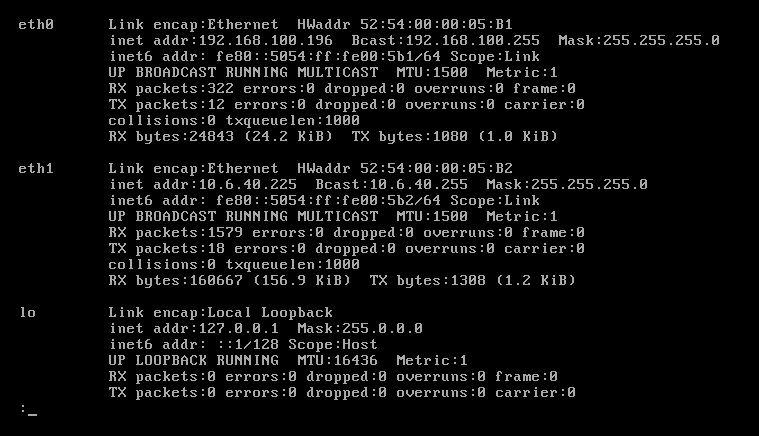
\includegraphics[width=10cm]{screenshots/ifconfig/ifconfig.png}}
\end{figure}

\newpage
\subsection{Instalación de \textit{httpd}}
Para iniciar la instalación del demonio \textbf{\textit{httpd}}, se utilizará el comando \textit{Yum}\footnote{https://access.redhat.com/es/solutions/238003} o Yellow dog Update, Modified, que es un gestor de paquetes desarrollado por la Universidad de Duke University para mejorar la instalación de paquetes RPMs utilizados entre otros, por Red Hat y CentOS. Para hacer lo anterior, se ejecutará el siguiente comando: \textbf{\textit{yum install httpd}}. El proceso, se detalla a continuación.
 \\[2cm]

\begin{figure}[ht]
\floatbox[{\capbeside\thisfloatsetup{capbesideposition={right,top},capbesidewidth=7cm}}]{figure}[\FBwidth]
{\caption{Yum automáticamente determinará qué paquetes adicionales deben ser descargados,  y así satisfacer las dependencias de \textit{httpd} . Para confirmar y continuar con el proceso, habrá que escribir \textit{``y''}.}\label{fig:dependencias}}
{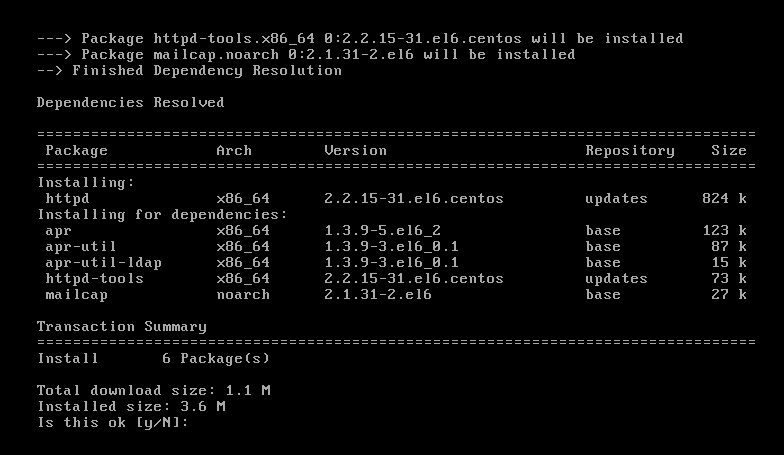
\includegraphics[width=10cm]{screenshots/httpd-install/lista-dependencias.png}}
\end{figure}


\begin{figure}[ht]
\floatbox[{\capbeside\thisfloatsetup{capbesideposition={left,top},capbesidewidth=7cm}}]{figure}[\FBwidth]
{\caption{Luego de confirmar y aceptar, se procederá a la descarga de los paquetes necesarios para completar la instalación.}\label{fig:descargando}}
{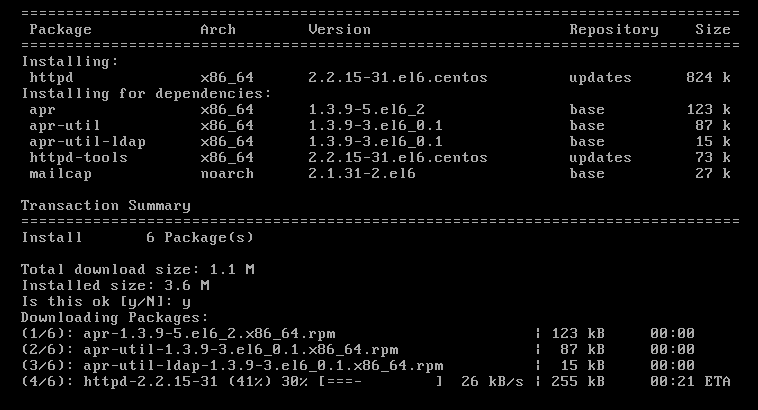
\includegraphics[width=10cm]{screenshots/httpd-install/descargando-paquetes.png}}
\end{figure}

\begin{figure}[ht]
\floatbox[{\capbeside\thisfloatsetup{capbesideposition={right,top},capbesidewidth=7cm}}]{figure}[\FBwidth]
{\caption{Completada la descarga, se presenta una lista de los paquetes necesarios que se instalarán. Además, se deberá confirmar la importación de la llave GPG de CentOS. Para continuar, aceptar con \textit{``y''}.}\label{fig:gpgKey}}
{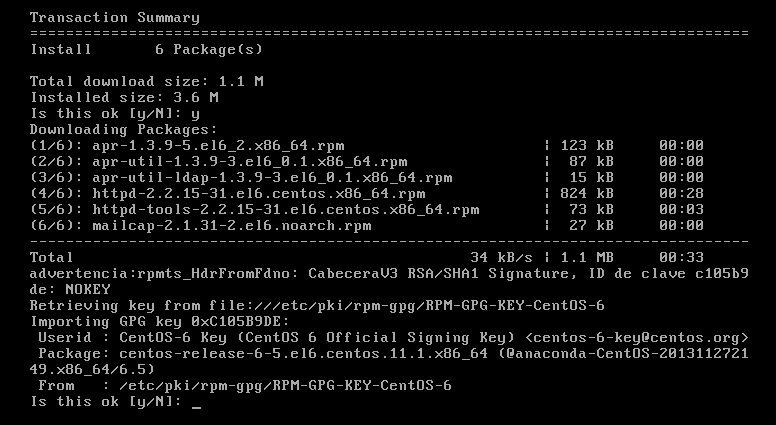
\includegraphics[width=10cm]{screenshots/httpd-install/aceptar-gpg-key.png}}
\end{figure}

\begin{figure}[ht]
\floatbox[{\capbeside\thisfloatsetup{capbesideposition={left,top},capbesidewidth=7cm}}]{figure}[\FBwidth]
{\caption{Luego de confirmar y aceptar los cambios, se llevará a cabo la instalación de los paquetes en el sistema.}\label{fig:instalando}}
{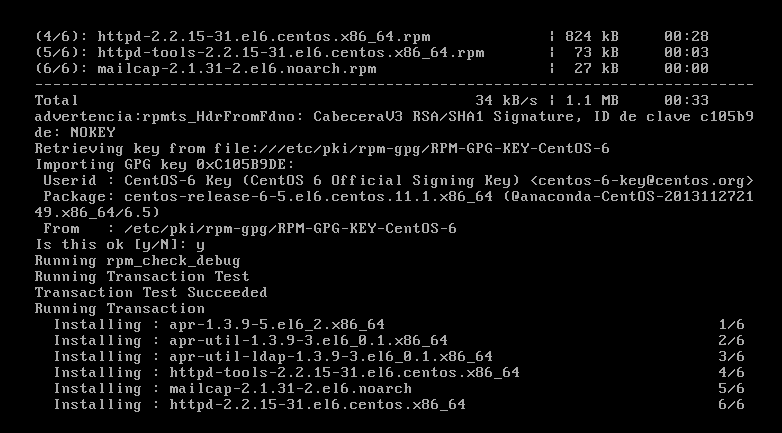
\includegraphics[width=10cm]{screenshots/httpd-install/instalando.png}}
\end{figure}

\begin{figure}[ht]
\floatbox[{\capbeside\thisfloatsetup{capbesideposition={right,top},capbesidewidth=7cm}}]{figure}[\FBwidth]
{\caption{La instalación de \textit{httpd} ha sido completada. Se presenta una lista con el paquete de \textit{httpd} instalado, además de sus dependencias.}\label{fig:terminado}}
{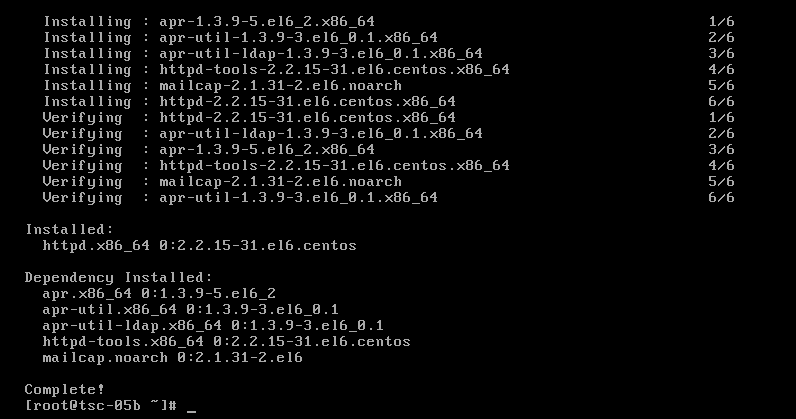
\includegraphics[width=10cm]{screenshots/httpd-install/terminado.png}}
\end{figure}

\clearpage

\subsection{Verificación del estado de \textit{httpd}}
Para comprobar que todo está en orden posterior a la instalación, se ejecuta el comando \textbf{yum info httpd}, con tal de obtener información acerca del estado del paquete \textit{httpd}.

\begin{figure}[ht]
\floatbox[{\capbeside\thisfloatsetup{capbesideposition={right,top},capbesidewidth=7cm}}]{figure}[\FBwidth]
{\caption{Comprobación de que el paquete ha sido instalado. Se muestra entre otras cosas, la versión del paquete, el tamaño en disco que ocupa y la arquitectura.}\label{fig:httpdInfo}}
{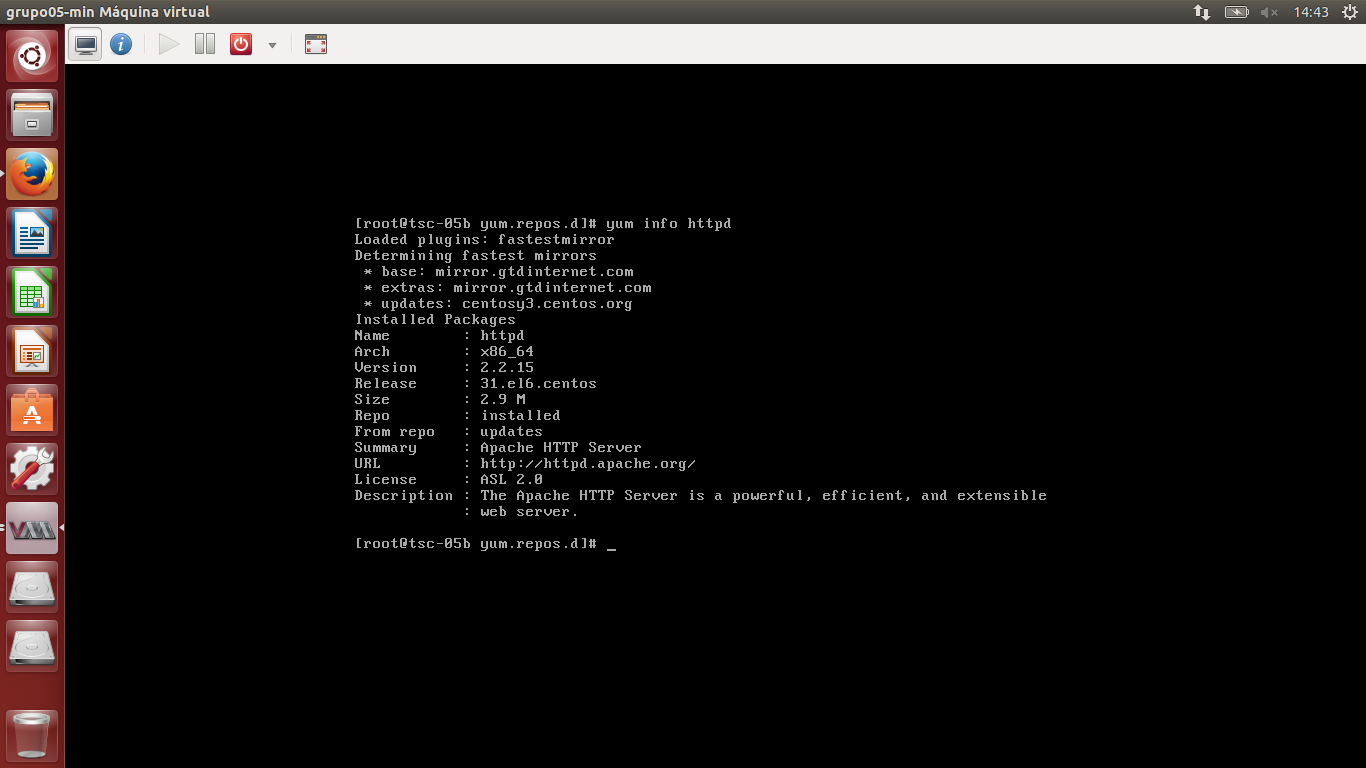
\includegraphics[width=10cm]{screenshots/httpd-install/yum-info-httpd.png}}
\end{figure}

\subsection{Configuración de \textit{httpd}}
El siguiente paso consiste en configurar la partida del servidor \textit{httpd} al encender el equipo o iniciar la máquina virtual. Para esto se utilizará la herramienta \textit{chkconfig} \footnote{http://access.redhat.com/documentation/en-US/Red\_Hat\_Enterprise\_Linux/6/html/Deployment\_Guide/s2-services-chkconfig.html}, utilidad que permite especificar en qué niveles de ejecución o \textit{run levels}\footnote{https://access.redhat.com/documentation/en-US/Red\_Hat\_Enterprise\_Linux/6/html/Installation\_Guide/s1-boot-init-shutdown-sysv.html} se iniciará un servicio. 

\begin{figure}[ht]
\floatbox[{\capbeside\thisfloatsetup{capbesideposition={left,top},capbesidewidth=7cm}}]{figure}[\FBwidth]
{\caption{Al ejecutar \textit{chkconfig}, se presetará una lista con todos los servicios del sistema y sus estados (activo o inactivo), en cada uno de los siete niveles de ejecución. Para el caso de \textit{httpd}, este se encuentra en estado inactivo en todos los niveles de ejecución.}\label{fig:httpdOff}}
{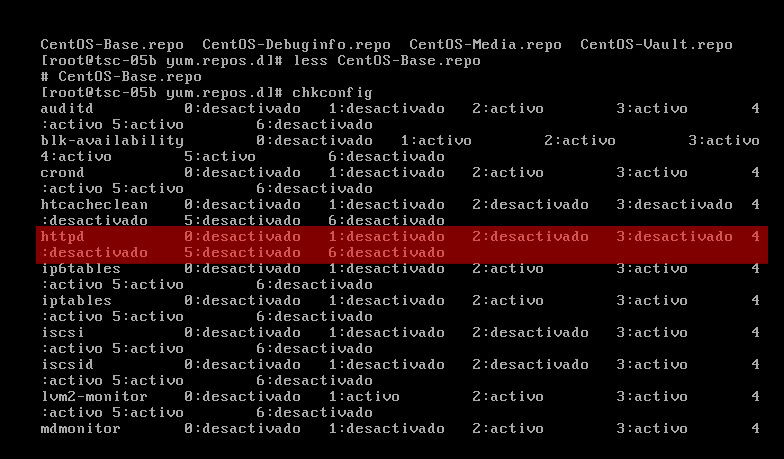
\includegraphics[width=10cm]{screenshots/httpd-run/chkconfig-httpd-off.png}}
\end{figure}

\clearpage

\begin{figure}[ht]
\floatbox[{\capbeside\thisfloatsetup{capbesideposition={right,top},capbesidewidth=6cm}}]{figure}[\FBwidth]
{\caption{Para activar un servicio, \textit{httpd} en este caso, en los niveles 2,3,4 y 5, se deberá tipear el comando \textit{chkconfig httpd on}. Al ejecutar \textit{chkconfig} nuevamente, se mostrará el resultado final en la Figura \ref{fig:httpdOn}. Los \textit{run levels} 0 (de apagado), 1 (modo de texto de un solo usuario) y 6 (de reinicio), se encuentran desactivados.}\label{fig:httpdOn}}
{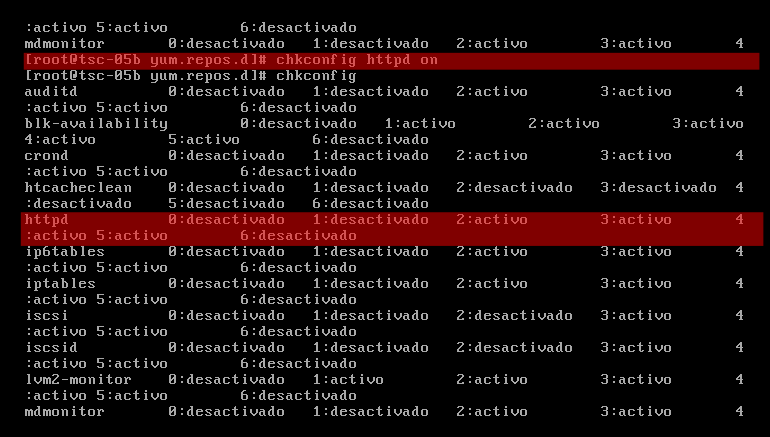
\includegraphics[width=11cm]{screenshots/httpd-run/chkconfig-httpd-on.png}}
\end{figure}


\subsection{Puesta en marcha y prueba}
Para poner en ejecución servidor \textit{httpd}, se utilizará \textit{service}\footnote{https://access.redhat.com/documentation/en-US/Red\_Hat\_Enterprise\_Linux/6/html/Deployment\_Guide/s1-services-running.html}, herramienta que permite inciar, detener o reiniciar los servicios desde el directorio \textbf{/etc/init.d/}. 

\begin{figure}[ht]
\floatbox[{\capbeside\thisfloatsetup{capbesideposition={left,top},capbesidewidth=7cm}}]{figure}[\FBwidth]
{\caption{Para iniciar el servicio \textit{httpd}, ejecutar el comando \textit{service httpd start}.}\label{fig:httpdServiceStart}}
{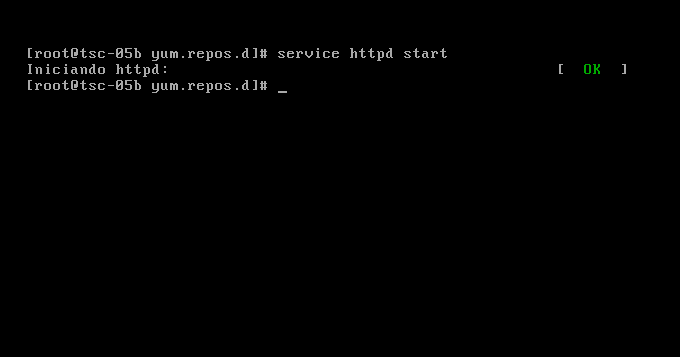
\includegraphics[width=10cm]{screenshots/httpd-run/service-httpd-start.png}}
\end{figure}

\begin{figure}[ht]
\floatbox[{\capbeside\thisfloatsetup{capbesideposition={right,top},capbesidewidth=7cm}}]{figure}[\FBwidth]
{\caption{Para comprobar el estado del servidor \textit{httpd}, se ejecutará el comando \textit{service httpd status}. Como puede verse en la figura, el servicio se encuentra en plena ejecución}\label{fig:httpdServiceStatus}}
{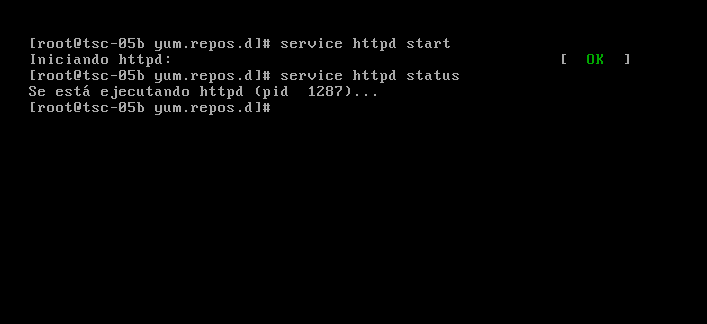
\includegraphics[width=10cm]{screenshots/httpd-run/service-httpd-status.png}}
\end{figure}

\newpage
\subsection{Permisos de archivos}
Es necesario verificar el nivel de acceso a archivos desde el sistema operativo, comprobando el estado de \textit{SELinux}\footnote{http://web.mit.edu/rhel-doc/4/RH-DOCS/rhel-rg-es-4/ch-selinux.html}, módulo de seguridad para el kernel Linux que proporciona el mecanismo para soportar políticas de seguridad para el control de acceso.
\begin{figure}[ht]
\floatbox[{\capbeside\thisfloatsetup{capbesideposition={right,top},capbesidewidth=7cm}}]{figure}[\FBwidth]
{\caption{Para chequear el estatus de \textit{SELinux}, se utiliza el comando \textit{getenforce}. Este comando retorna Enforcing, Permissive, o Disabled.}\label{fig:getenforce}}
{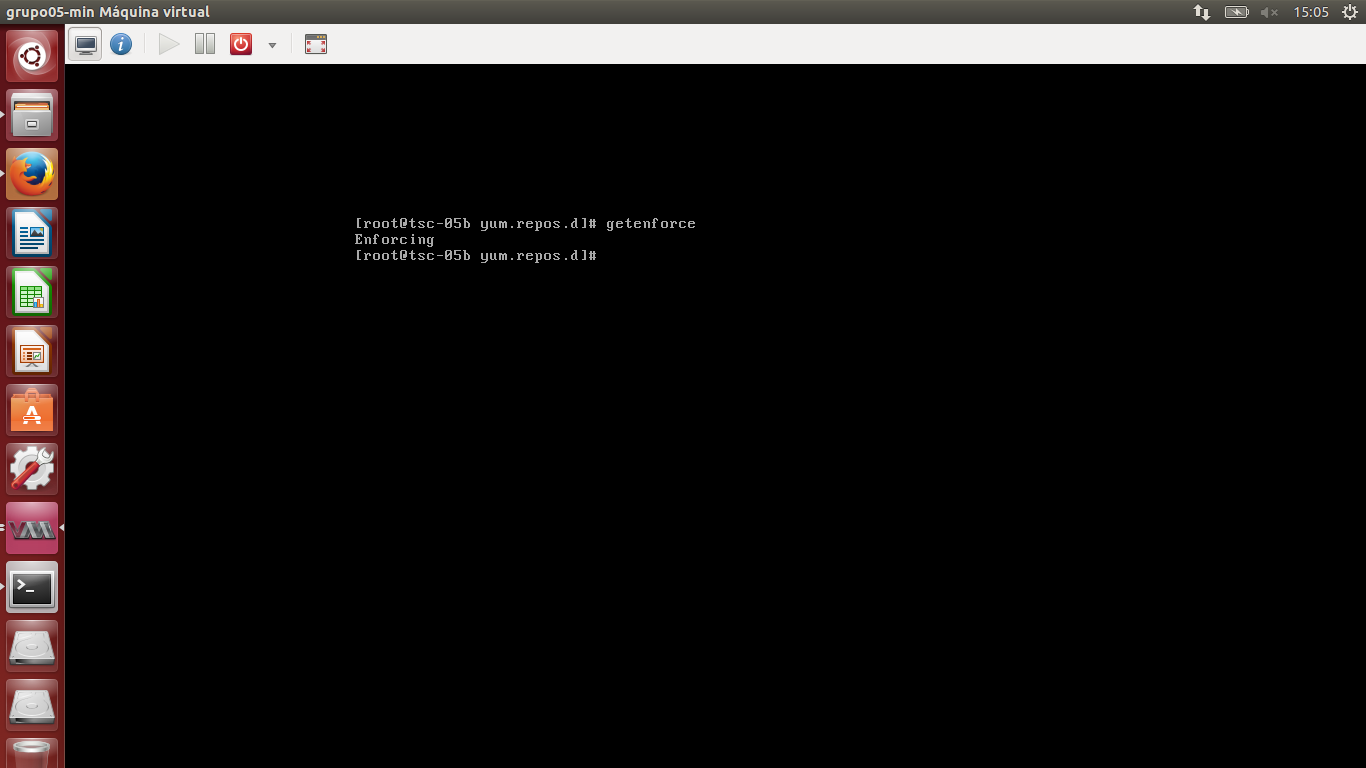
\includegraphics[width=10cm]{screenshots/permissions/getenforce.png}}
\end{figure}

\begin{figure}[ht]
\floatbox[{\capbeside\thisfloatsetup{capbesideposition={left,top},capbesidewidth=7cm}}]{figure}[\FBwidth]
{\caption{Para configurar un determinado estado de \textit{SELinux}, se utiliza el comando \textit{setenforce}. En este caso se configura en estado \textit{permissive}, donde las políticas de \textit{SELinux} no son aplicadas, pero las negaciones son todavía registradas para las acciones que habrían sido denegadas si se está en modo \textit{enforcing}.}\label{fig:setPermissive}}
{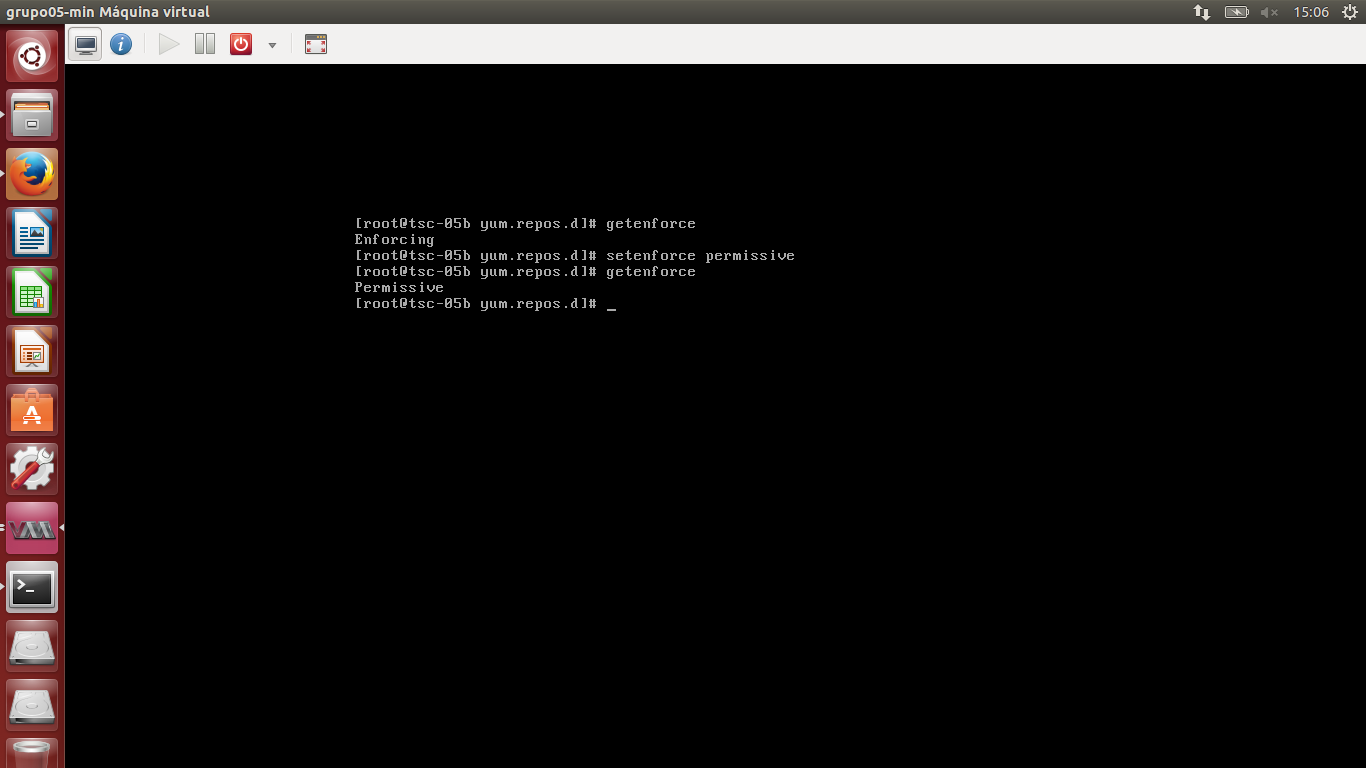
\includegraphics[width=10cm]{screenshots/permissions/set-permissive.png}}
\end{figure}


\subsection{Configuración firewall}
Para posibilitar las conexiones al puerto 80, utilizado por el servidor, es necesario modificar las reglas \textit{IPtables}, firewall utilizado para gestionar las conexiones en Linux. Para aquello, es necesario modificar el archivo de configuración \textbf{iptables}, que se encuentra en el directorio \textbf{/etc/sysconfig/}. 

\begin{figure}[ht]
\floatbox[{\capbeside\thisfloatsetup{capbesideposition={right,top},capbesidewidth=7cm}}]{figure}[\FBwidth]
{\caption{Estado inicial del archivo de configuración de iptables. Solo el puerto 22 (ssh) tiene permisos de acceso.}\label{fig:iptablesBefore}}
{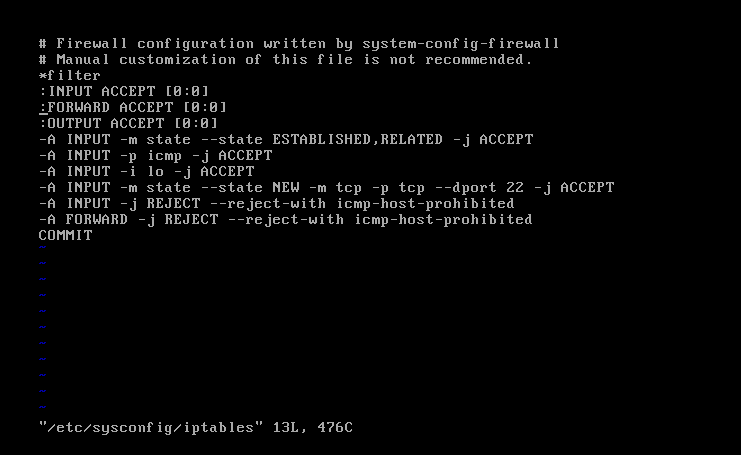
\includegraphics[width=10cm]{screenshots/iptables-config/vi-iptables-before.png}}
\end{figure}

\clearpage

\begin{figure}[ht]
\floatbox[{\capbeside\thisfloatsetup{capbesideposition={left,top},capbesidewidth=7cm}}]{figure}[\FBwidth]
{\caption{Estado del archivo de configuración de iptables, luego de agregar las nuevas reglas para el puerto 80 y posibilitar el uso del protocolo de transferencia de hipertexto (HTTP).}\label{fig:iptablesAfter}}
{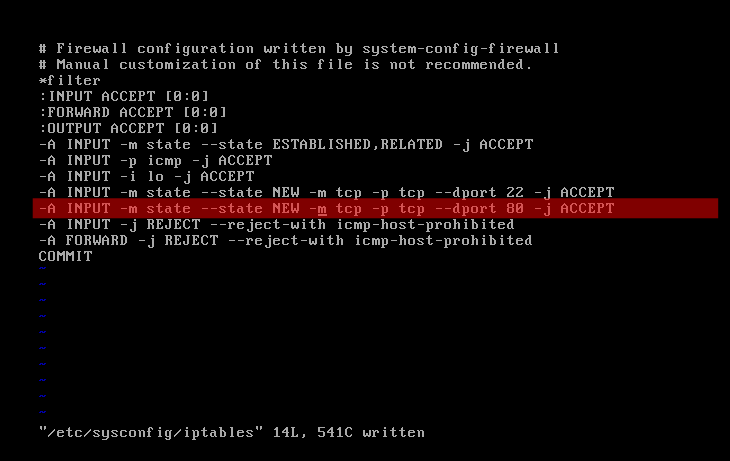
\includegraphics[width=10cm]{screenshots/iptables-config/vi-iptables-port-80-enabled.png}}
\end{figure}

\begin{figure}[ht]
\floatbox[{\capbeside\thisfloatsetup{capbesideposition={right,top},capbesidewidth=7cm}}]{figure}[\FBwidth]
{\caption{Para que los cambios surtan efecto, es preciso reiniciar el sistema o simplemente reiniciar \textit{iptables}. Se opta por esto último, por lo que se ejecuta el comando \textit{service iptables restart}.}\label{fig:iptablesRestart}}
{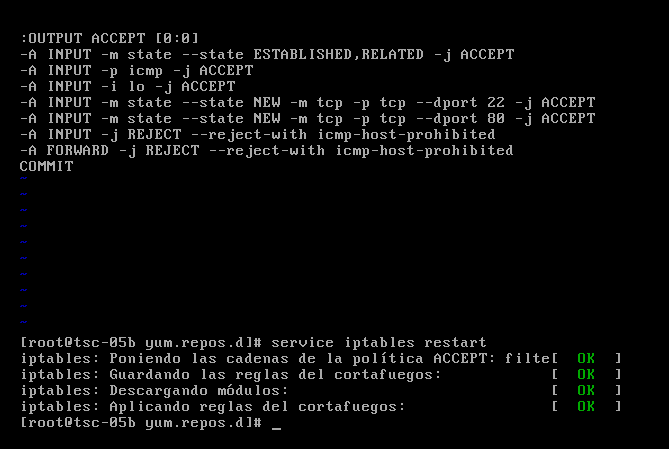
\includegraphics[width=10cm]{screenshots/iptables-config/iptables-restart.png}}
\end{figure}


Ahora con todo esto configurado, se debería ser capaz de conectar al servidor desde otra máquina, lo que se muestra en la próxima sección.

\subsection{Conexión al servidor mediante Telnet}
\textit{Telnet} es utilizado para comunicarse con otro servidor, utilizando el protocolo TELNET. Su uso ha sido descontinuado dada su baja seguridad, sin embargo, se utiliza en esta experiencia con fines experimentales.\par
Dado que por defecto \textit{Telnet} no viene con la versión de CentOS instalada, se debe instalar con la herramienta \textit{yum}, como puede verse en la Figura \ref{fig:telnetInstall}.
\clearpage

\begin{figure}[ht]
\floatbox[{\capbeside\thisfloatsetup{capbesideposition={left,top},capbesidewidth=7cm}}]{figure}[\FBwidth]
{\caption{Instalación de \textit{telnet}, mediante la ejecución del comando \textit{yum install telnet}.}\label{fig:telnetInstall}}
{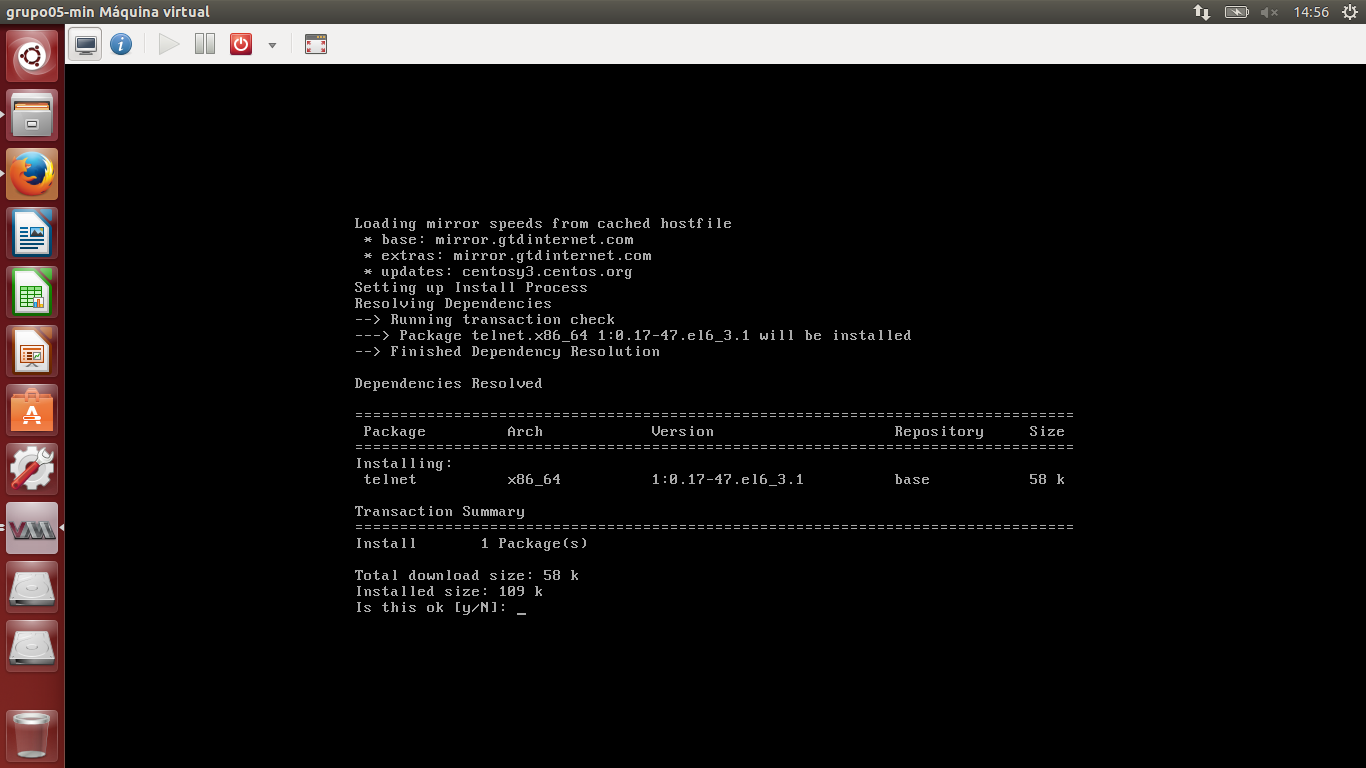
\includegraphics[width=10cm]{screenshots/telnet-install/telnet-install.png}}
\end{figure}

\begin{figure}[ht]
\floatbox[{\capbeside\thisfloatsetup{capbesideposition={right,top},capbesidewidth=7cm}}]{figure}[\FBwidth]
{\caption{Instalación de \textit{Telnet} finalizada.}\label{fig:telnetInstalled}}
{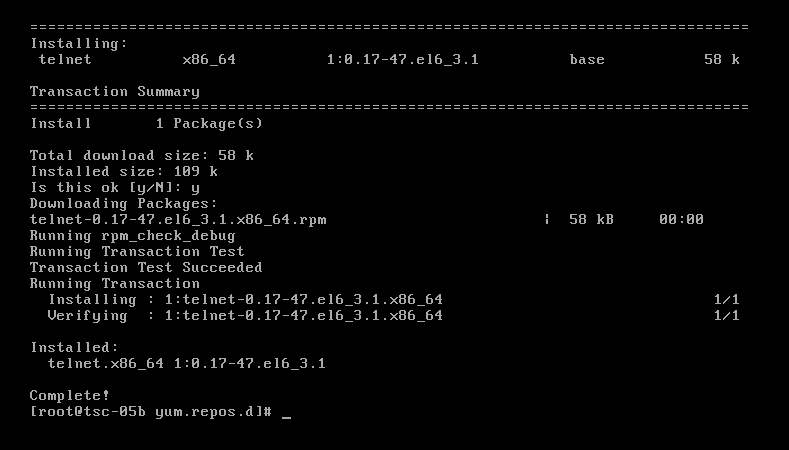
\includegraphics[width=10cm]{screenshots/telnet-install/telnet-instalacion-completa.png}}
\end{figure}

Ahora, para comprobar el funcionamiento de \textit{telnet}, se realizará una petición HTTP GET al puerto 80 al localhost o de la máquina virtual a si misma.

\begin{figure}[ht]
\floatbox[{\capbeside\thisfloatsetup{capbesideposition={left,top},capbesidewidth=7cm}}]{figure}[\FBwidth]
{\caption{Petición HTTP \textit{GET} al puerto 80 del localhost, utilizando \textit{telnet}. El resultado es una página html en formato de texto plano.}\label{fig:telnetLocalhost80}}
{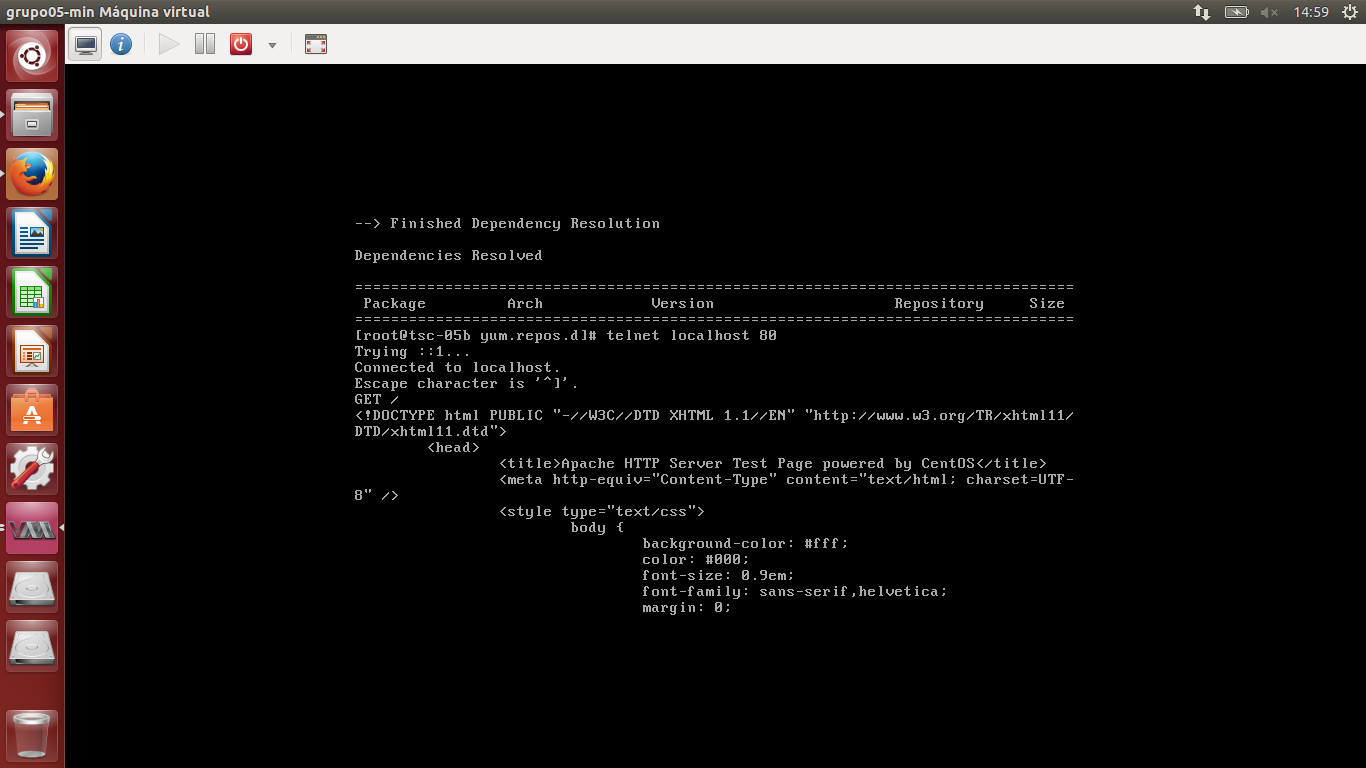
\includegraphics[width=10cm]{screenshots/communication/telnet-get-80.png}}
\end{figure}

De forma análoga, también podemos realizar esto desde la máquina anfitrión, teniendo en consideración que ahora debemos ingresar la IP de la máquina mínima en lugar de localhost, o sea, debemos ingresar \textbf{telnet 10.6.40.225 80}

\clearpage

\begin{figure}[ht]
\floatbox[{\capbeside\thisfloatsetup{capbesideposition={right,top},capbesidewidth=7cm}}]{figure}[\FBwidth]
{\caption{Petición HTTP \textit{GET}, desde el equipo anfitrión de virtualización, a la máquina virtual mínima. El resultado es una página html en formato de texto plano.}\label{fig:telnetHostToMin}}
{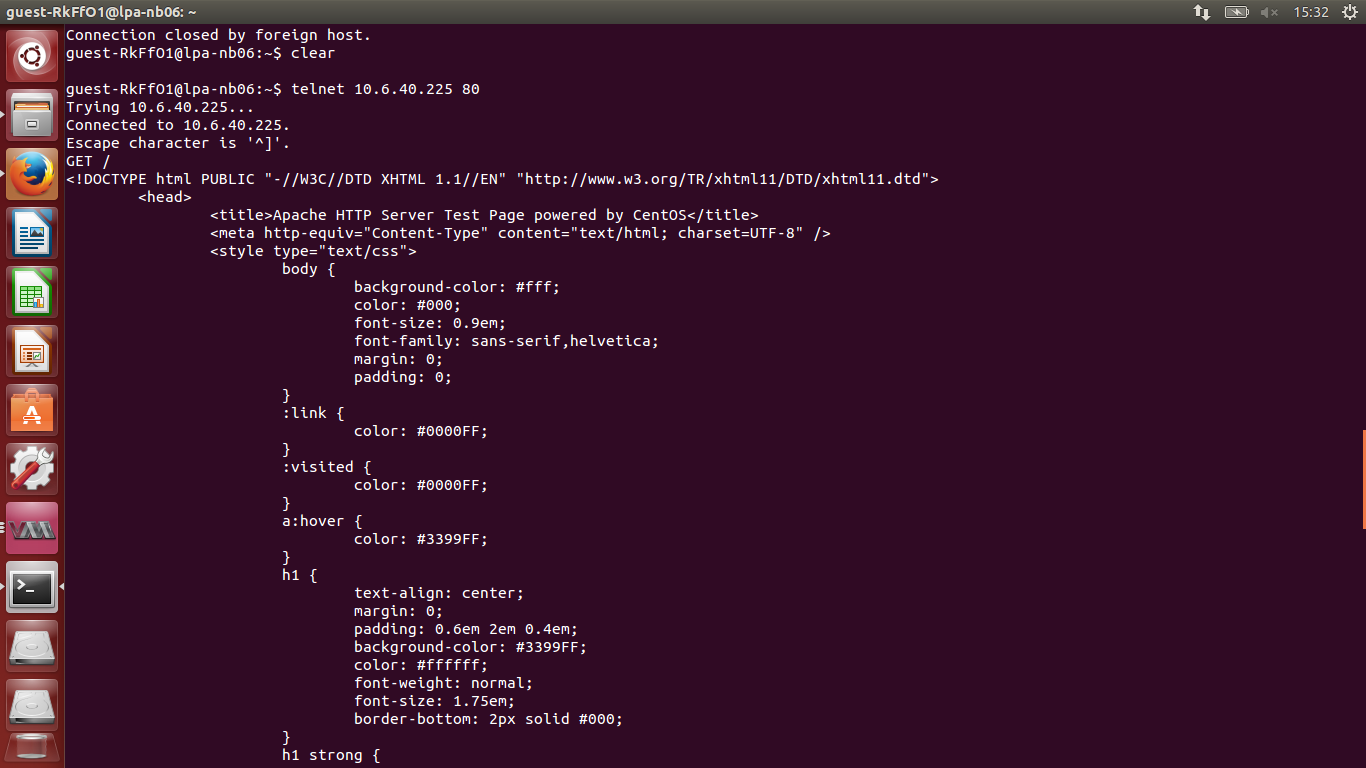
\includegraphics[width=10cm]{screenshots/communication/get-to-min-from-host.png}}
\end{figure}

\subsection{Conexión al servidor mediante browser}
Finalmente, se desea conectar al servidor mediante un explorador web con interfaz gráfica. Nuevamente desde la máquina anfitrión abrimos un navegador cualquiera, e ingresamos en la barra de direcciones la dirección IP del servidor, o sea, \textbf{10.6.40.225}, dando como resultado la página por defecto de Apache.

\begin{figure}[ht]
\floatbox[{\capbeside\thisfloatsetup{capbesideposition={right,top},capbesidewidth=7cm}}]{figure}[\FBwidth]
{\caption{Desde el navegador web Firefox, viendo la página web de prueba del servidor \textit{httpd}.}\label{fig:browserHostToMin}}
{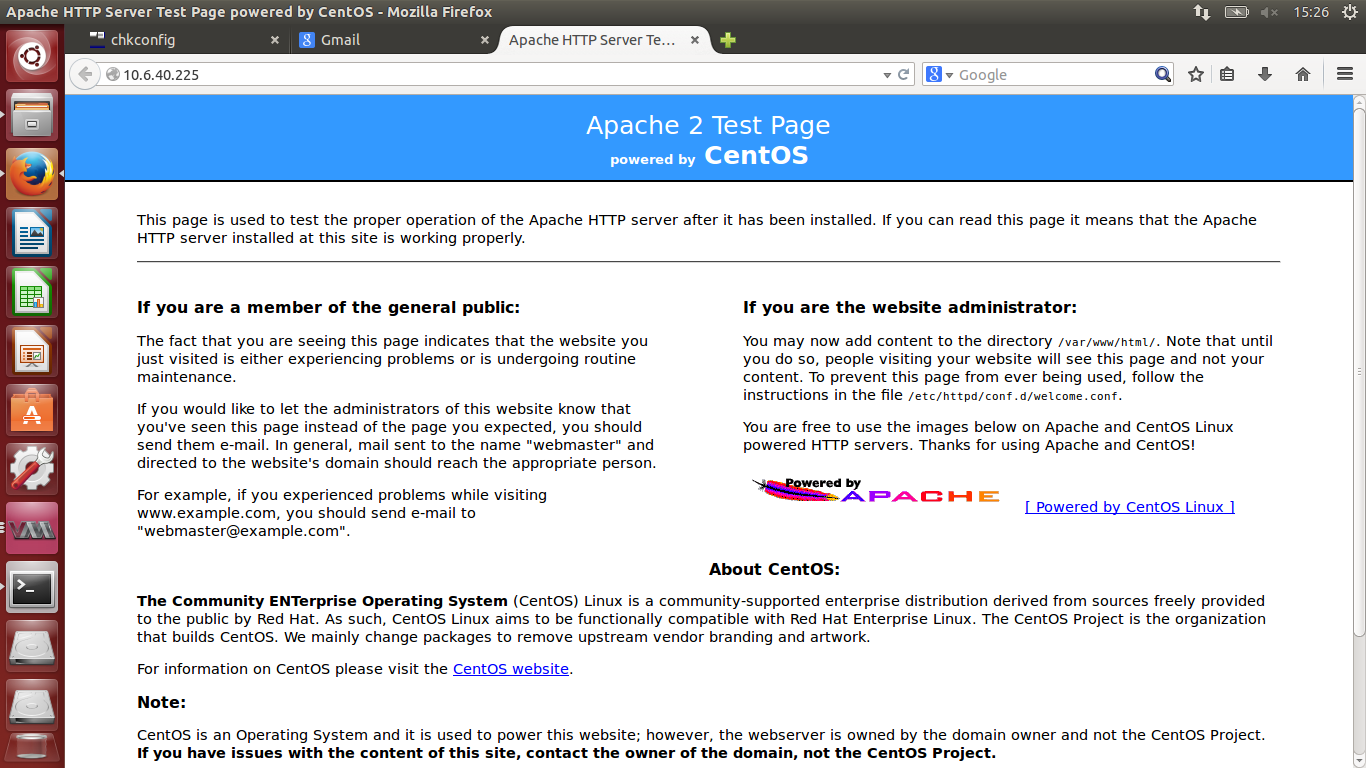
\includegraphics[width=10cm]{screenshots/communication/host-browser-to-min.png}}
\end{figure}

\section{Conclusión}
Se logró instalar de forma satisfactoria el servidor web Apache httpd, mediante la utilización del gestor de paquetes de CentOS, \textit{yum}. Posteriormente, se realizó el proceso básico de configuración de un demonio de sistema, especificando los \textit{run levels} en que se encontrará activo, asi como también el proceso de inicio, detención y reinicio de un servicio de sistema con el comando \textit{service}. Además, se aprendieron las nociones básicas del firewall de Linux \textit{IPTables},  y su configuración, para así posibilitar la comunicación de varios equipos, utilizando distintos protocolos.

\end{document}
